\documentclass[a4paper, 11pt]{article}
\usepackage[top=3cm, bottom=3cm, left = 2cm, right = 2cm]{geometry} 
\geometry{a4paper} 
\usepackage[utf8]{inputenc}
\usepackage{textcomp}
\usepackage{graphicx} 
\usepackage{amsmath,amssymb}  
\usepackage{bm}  
% \usepackage{fontspec} % Required for using system fonts (including Roboto)
% \setmainfont{Roboto} % Set Roboto as the main font


\usepackage{memhfixc} 
\usepackage{pdfsync}  
\usepackage{array}
\usepackage{xcolor}
\usepackage{tcolorbox}
\usepackage{graphicx}
\usepackage{wrapfig}

% \usepackage{fancyhdr}
% \pagestyle{fancy}

\title{CS378 - Computer Networks Lab \\ Lab 01 Submission}
\author{Omkar Shirpure (22B0910)}
%\date{}

\begin{document}
\maketitle
\vspace{5cm}
\tableofcontents

\newpage
\section{}
\vspace{1cm}
\begin{center}
    \resizebox{17cm}{10.5cm}{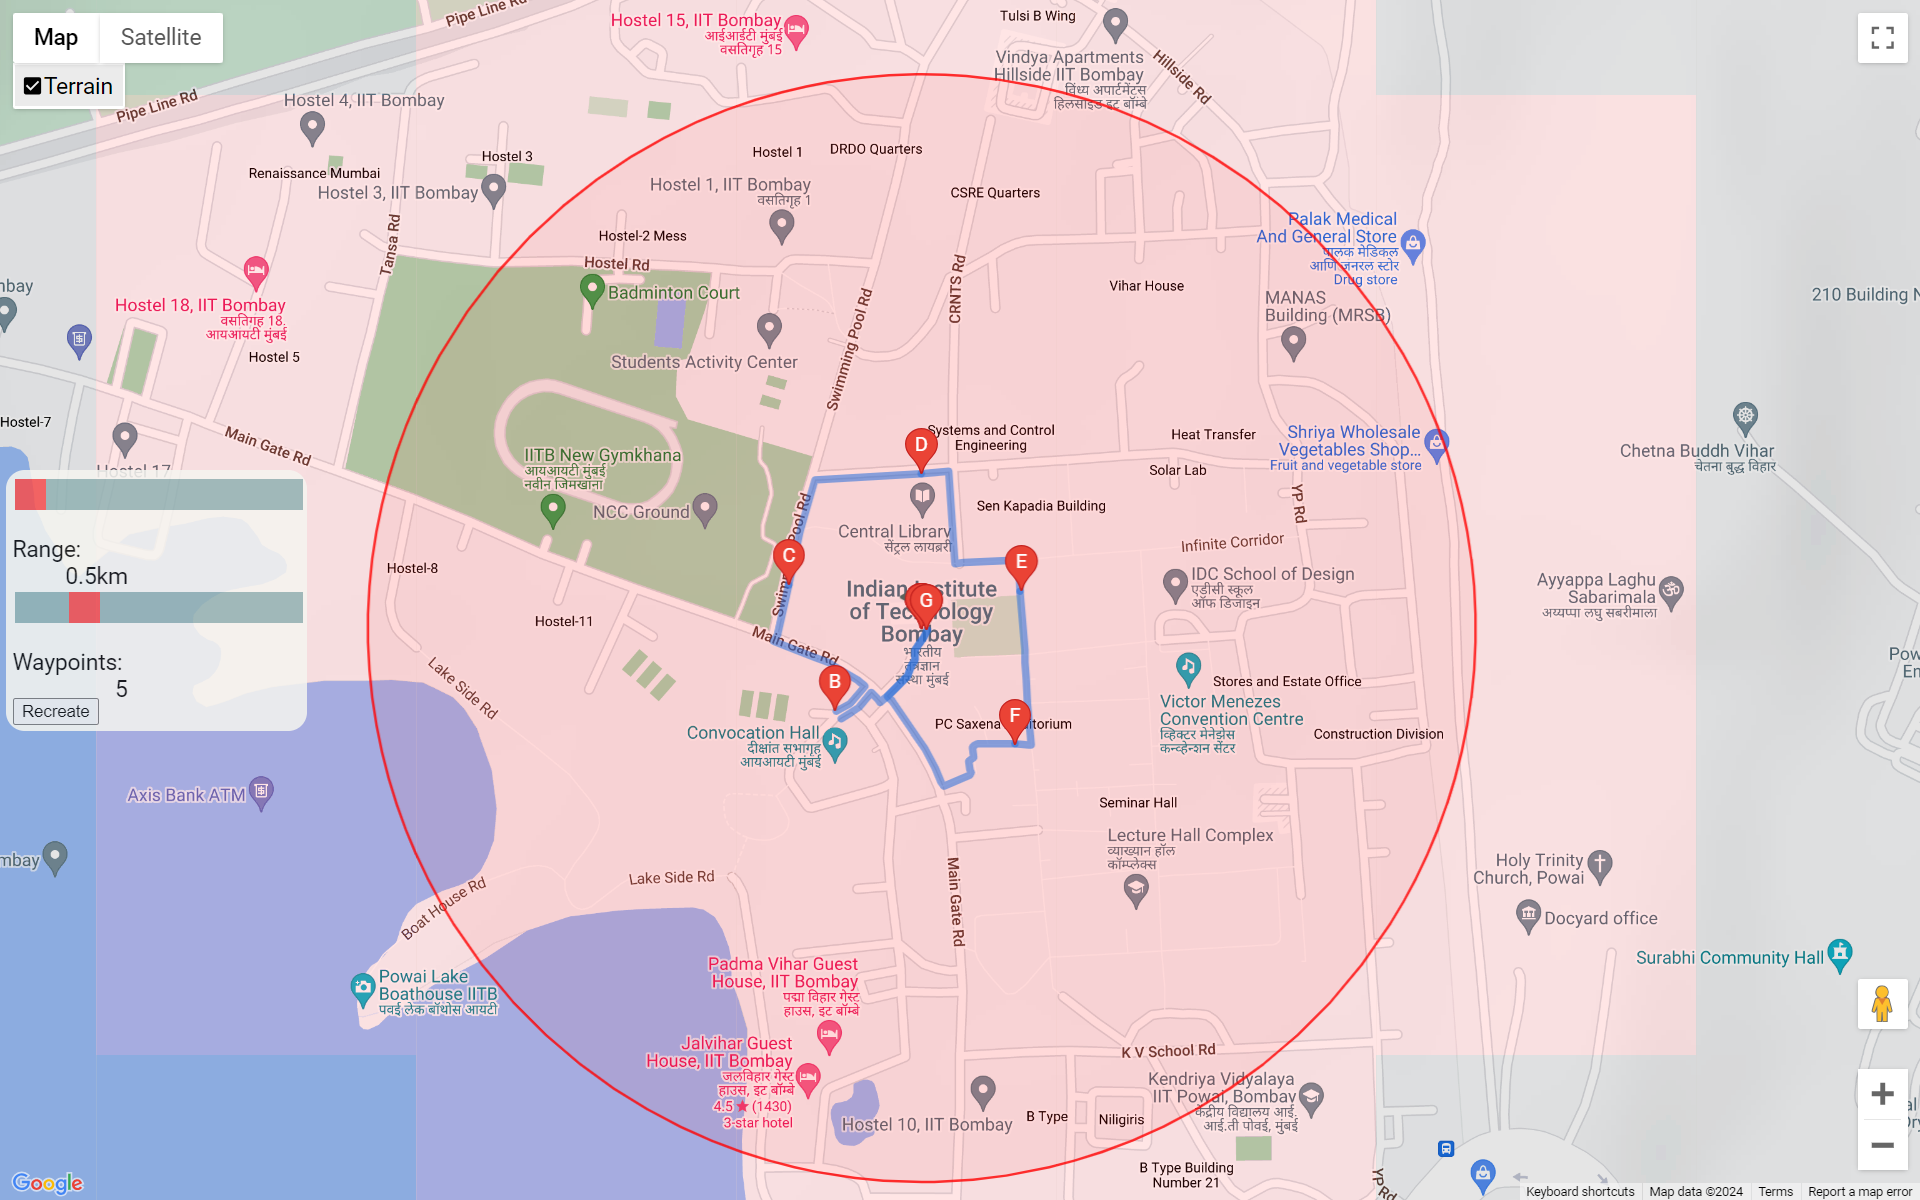
\includegraphics{Lab01/imgs/walk.png}}
\end{center}

\vspace{1cm}
The generated path's location was IIT Bombay with range of $0.5$ KM with 5 Waypoints. \\

\begin{tcolorbox}[colback=gray!20, colframe=gray!80]
    \textbf{Note}: The waypoints were labelled starting from B-C-D... (for unknown reason) and for the sake of convention, we'll use the same labels throughout the report.
\end{tcolorbox}

\newpage
\section{}
\vspace{1cm}
\begin{center}
    \resizebox{12cm}{15cm}{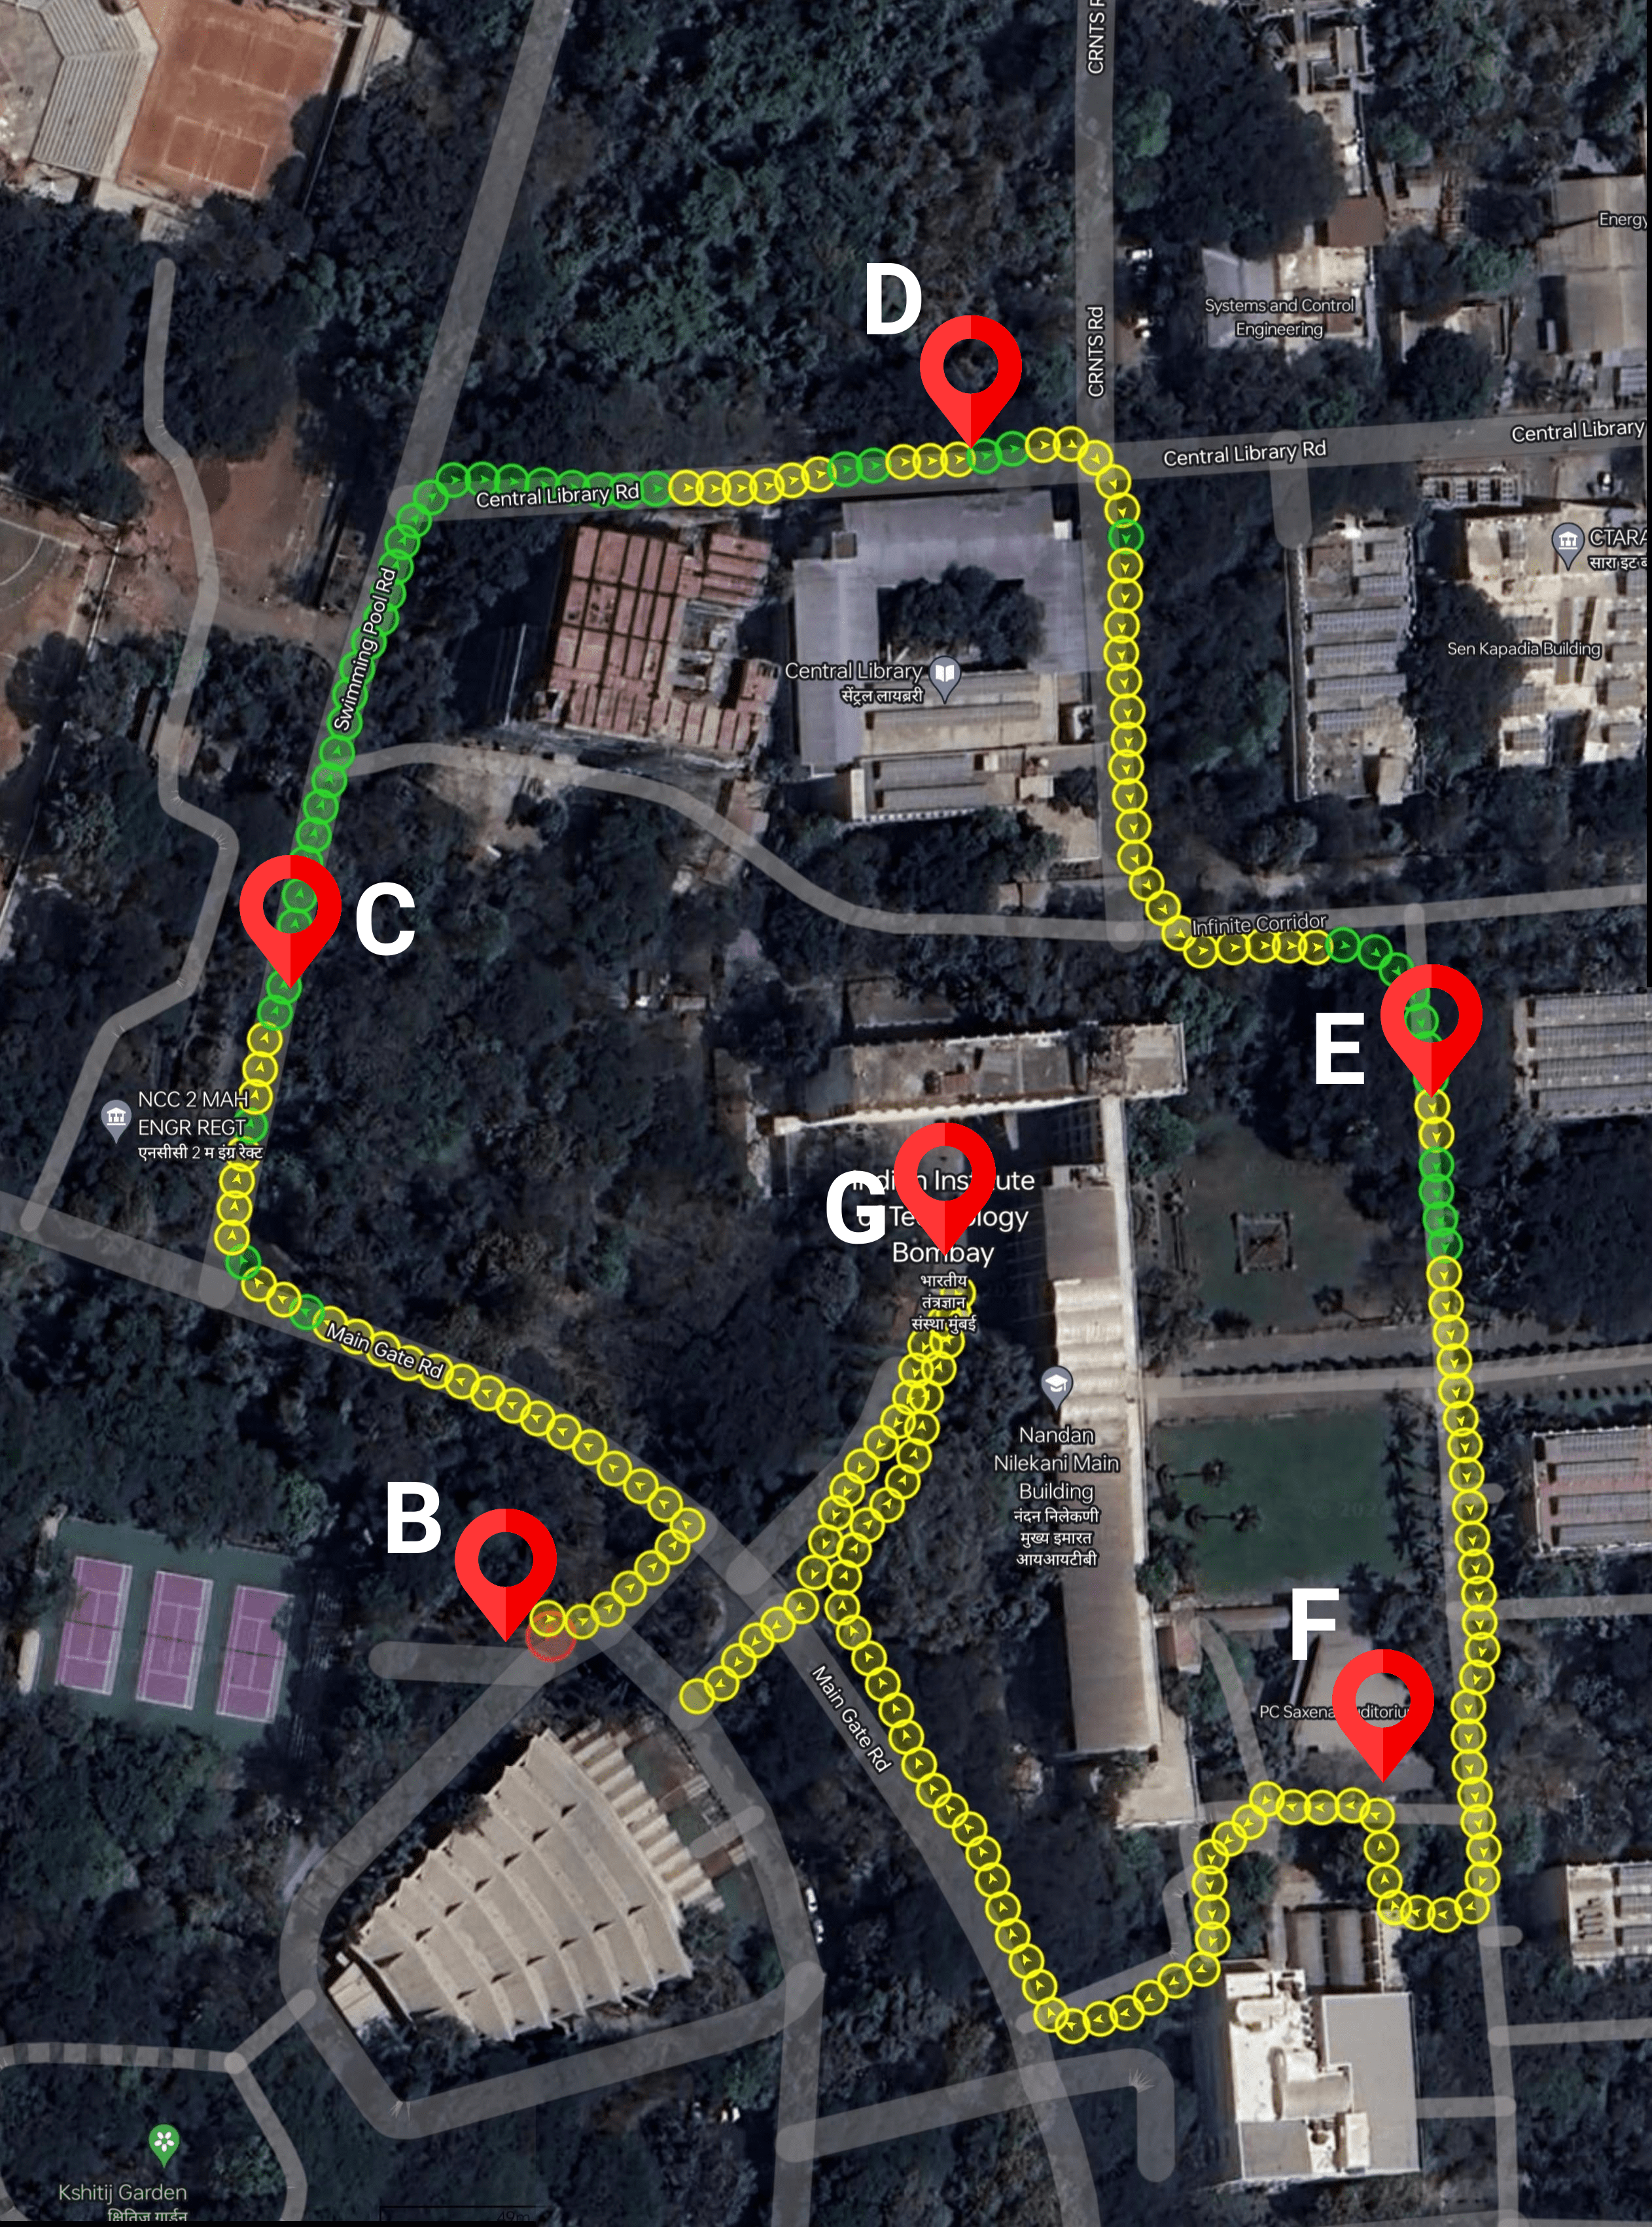
\includegraphics{Lab01/imgs/signal_strengths_labelled.png}}
\end{center}
\vspace{0.5cm}
The signal strengths (RSRP) and the colors corresponding in the map are as follows (in dBm): 
\begin{itemize}
    \item \textcolor{green}{\textbf{Green}} (good):\hspace{2.93cm} $x \geq -84$
    \item \textcolor{yellow}{\textbf{Yellow}} (not bad): \hspace{1.15cm}$-85 \geq x \geq -104$
    \item \textcolor{red}{\textbf{Red}} (bad): \hspace{2.15cm}$-105 \geq x$
\end{itemize}
\vspace{5pt}

\section{}
The network provider used for the measurements is \textbf{Airtel} (Bharti Airtel Limited).

\newpage
\section{}
The unique base-stations the phone was connected with \textbf{approximate} locations are as follows:

\vspace{0.5cm}

\begin{center}
\renewcommand{\arraystretch}{1.5} % Adjust row height
    \begin{tabular}{|c|c|}
        \hline
        \hspace{0.5cm}\textbf{eNodeBID}\hspace{0.5cm} & \hspace{0.5cm}\textbf{Location}\hspace{0.5cm} \\
        \hline
        \hspace{0.5cm}906129\hspace{0.5cm} & \hspace{0.5cm}Path B-C\hspace{0.5cm} \\
        \hline
        \hspace{0.5cm}901396\hspace{0.5cm} & \hspace{0.5cm}Path C-D\hspace{0.5cm} \\
        \hline
        \hspace{0.5cm}651698\hspace{0.5cm} & \hspace{0.5cm}Path D-E-F-G\hspace{0.5cm} \\
        \hline
    \end{tabular}
\end{center}

% \newpage
\vspace{0.25cm}

\section{}

Throughout the path, the signal strength generally ranged from good to medium, but there were certain areas where it dropped to poor levels. \\
% \vspace{-1cm}

\begin{wrapfigure}[6]{r}{0.3\textwidth} % [9] limits wrapping to 9 lines
    \centering
    \vspace{-0.95cm}
    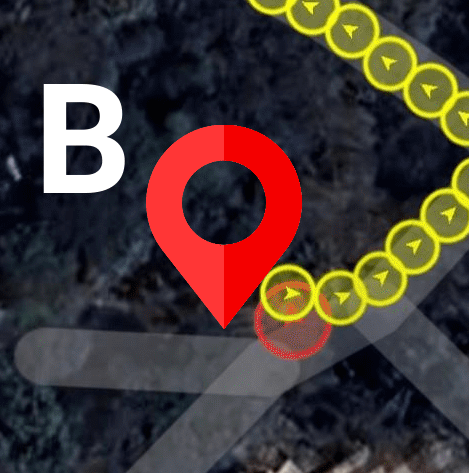
\includegraphics[width=0.21\textwidth]{Lab01/imgs/weak_signal_area.png}
    \caption{Map showing locations with weak signals.}
\end{wrapfigure}

The locations where weak signals were observed include:

\begin{itemize}
    \item \textbf{Location:} At the start of the path, near tag B.
    \item \textbf{Possible Causes:} The poor signal in this area could be majorly attributed to its low-lying position, and dense tree coverage. There could also be several other factors, like obstruction by the Convocation Hall on one side, etc. 
\end{itemize}

Multiple red points are denoted by a larger red blob.\\

\vspace{10pt}
The medium signal strength, indicated by yellow points, could be mainly due to sparse tree coverage (B-C), building obstructions (D-E, near G), covered corridors (near F), and elevation changes. \\
Signal strengths were higher in open areas, such as the right turns from C-D, B-C, and near E.

% \newpage
\vspace{10pt}
\section{}

At a fixed location, the values of the RSRA signal strength varies over time. The measurements taken over 1 minute are as follows:

\vspace{0.5cm}
\begin{center}
    {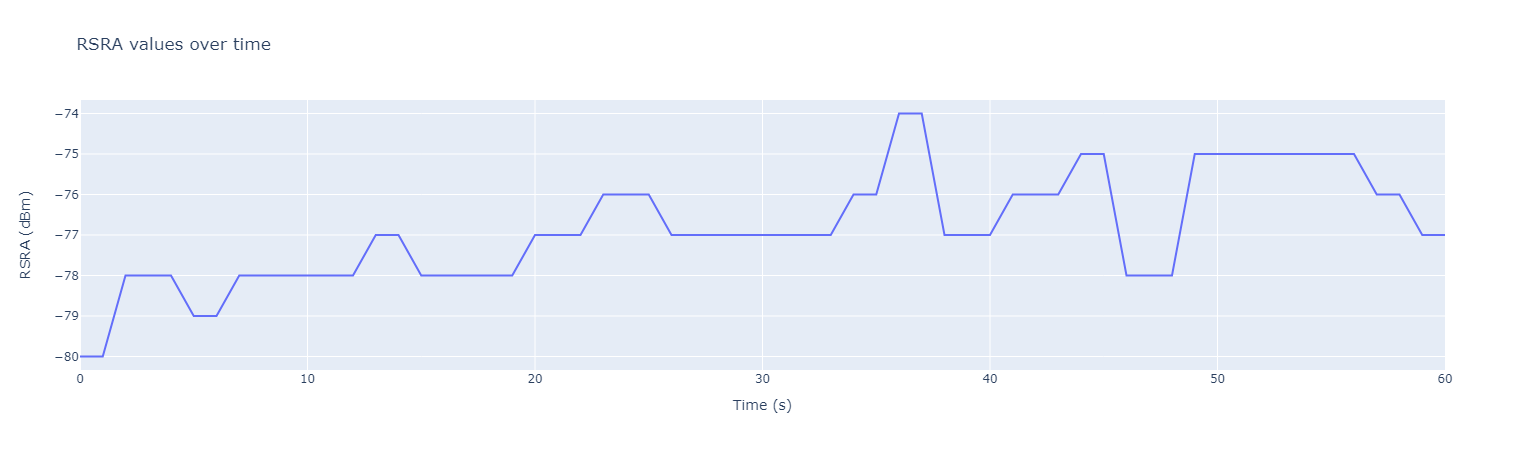
\includegraphics[width=17cm]{Lab01/imgs/rsra_plot.png}}
\end{center}

\end{document}
